\documentclass[11pt]{article}
\usepackage[T1]{fontenc}
\usepackage{lmodern}
\pdfglyphtounicode{parenleftbig}{0028}
\pdfglyphtounicode{parenrightbig}{0029}
\pdfglyphtounicode{parenleftBig}{0028}
\pdfglyphtounicode{parenrightBig}{0029}
\pdfgentounicode=1
\usepackage[margin=1.05in]{geometry}
\usepackage{amsmath,amssymb,amsthm,mathtools}
\usepackage{microtype}
\usepackage{enumitem}
\usepackage{xcolor}
\usepackage{tikz}
\usetikzlibrary{arrows.meta,positioning,calc}
\usepackage[hidelinks]{hyperref}
\hypersetup{pdftitle={A proof of Seymour's second-neighborhood conjecture},
 pdfauthor={OpenAI}, pdfsubject={Oriented graphs and finite relations}}
\pdftrailerid{}
\newtheorem{theorem}{Theorem}[section]
\newtheorem{lemma}[theorem]{Lemma}
\newtheorem{proposition}[theorem]{Proposition}
\newtheorem{corollary}[theorem]{Corollary}
\theoremstyle{remark}
\newtheorem{remark}[theorem]{Remark}
\newcommand{\abs}[1]{\lvert #1\rvert}
\DeclareMathOperator{\rank}{rank}
\DeclareMathOperator{\im}{im}
\DeclareMathOperator{\Arc}{Arc}
\DeclareMathOperator{\Non}{Non}
\newcommand{\R}{\mathbb R}
\newcommand{\unverified}[1]{\par\smallskip\noindent\fbox{\parbox{0.95\linewidth}{\textbf{Unverified step.} #1}}\par\smallskip}
\newcommand{\Step}[1]{\par\medskip\noindent\textbf{#1}\enspace}
\newcommand{\tp}{^{\mathsf T}}
\newcommand{\cR}{\mathcal R}
\newcommand{\cC}{\mathcal C}
\newcommand{\cM}{\mathcal M}
\newcommand{\cV}{\mathcal V}
\newcommand{\bu}{\mathbf u}
\newcommand{\bv}{\mathbf v}
\newcommand{\bx}{\mathbf x}
\newcommand{\by}{\mathbf y}
\newcommand{\be}{\mathbf e}
\newcommand{\tN}{\widetilde N}
\newcommand{\tF}{\widetilde F}
\title{A proof of Seymour's second-neighborhood conjecture}
\author{Rewritten for readability from the OpenAI manuscript of the same title}
\date{September 23, 2026}
\begin{document}
\maketitle
\begin{abstract}
We prove that every nonempty finite oriented graph has a vertex with at least
as many vertices at directed distance two as at directed distance one.
This resolves Seymour's second neighborhood conjecture positively.
\end{abstract}

\section{Introduction: the result and the plan}\label{sec:introduction}

\subsection{The main result}

An \emph{oriented graph} is a finite directed graph with no loops, no multiple
arcs, and no pair of opposite arcs. Its underlying undirected graph need
not be complete or connected. We write $v\to u$ when there is an arc from $v$ to $u$.
For a vertex \(v\), write
\[
 N_1^+(v)=\{u:v\to u\},\qquad
 N_2^+(v)=\{w\notin\{v\}\cup N_1^+(v):
                 \text{ there is a vertex }u\text{ with }v\to u\to w\}.
\]
Thus \(N_2^+(v)\) consists of the vertices at directed distance exactly two
from \(v\). Each vertex is counted once, regardless of the number of paths
reaching it.

\begin{theorem}\label{thm:main}
Every nonempty finite oriented graph has a vertex \(v\) such that
\[
 \abs{N_1^+(v)}\leq \abs{N_2^+(v)}.
\]
\end{theorem}

This is Seymour's second neighborhood conjecture. There is no
connectivity or degree hypothesis. A \emph{sink} (a vertex with
$N_1^+(v)=\varnothing$) satisfies the conclusion trivially, since then
$N_2^+(v)=\varnothing$ as well and $0\le 0$. Removing from $N_2^+(v)$ the
vertices already reached in one step is essential to the statement.

Sections~\ref{sec:weighted-consequences}
and~\ref{sec:directed-cycle-consequences} derive weighted forms and
consequences for short directed cycles. Section~\ref{sec:context} records
prior work.

\subsection{Image operators}

For a digraph \(D\) and a set \(S\) of its vertices, define
\[
 F_D(S)=\{y:\text{ there is }x\in S\text{ with }x\to y\},
 \qquad F_D^2(S)=F_D(F_D(S)).
\]
The operator \(F_D\) does \emph{not} subtract \(S\): $F_D(S)$ may meet $S$.
Clearly $F_D(S\cup S')=F_D(S)\cup F_D(S')$ and $F_D(\varnothing)=\varnothing$.
In an oriented graph,
\begin{equation}\label{eq:exact-second}
 N_1^+(v)=F_D(\{v\}),\qquad N_2^+(v)=F_D^2(\{v\})\setminus F_D(\{v\}).
\end{equation}
\emph{Proof of the second identity.} By definition $w\in F_D^2(\{v\})$ if and
only if $v\to u\to w$ for some $u$. Such a $w$ is never $v$, because
$v\to u$ and $u\to v$ would be opposite arcs. So removing
$\{v\}\cup N_1^+(v)$ from $F_D^2(\{v\})$ is the same as removing
$N_1^+(v)=F_D(\{v\})$.\hfill$\square$

\subsection{Proof at a glance}

Call a nonempty finite oriented graph a \emph{counterexample} if
$\abs{N_1^+(v)}>\abs{N_2^+(v)}$ for \emph{every} vertex $v$.
Theorem~\ref{thm:main} says that there is no counterexample. The proof is by
contradiction and has two halves, joined by a single inequality.

\paragraph{Half 1 (Section~\ref{sec:reduction}): from a counterexample to a
``strictly concave'' graph.}
If a counterexample exists, then there is an oriented graph $G$, all of
whose vertices have an in-neighbour, such that
\begin{equation}\label{eq:overview-concavity}
 \abs{U}+\abs{F_G^2(U)}<2\abs{F_G(U)}
 \qquad\text{for every }\varnothing\ne U\subsetneq V(G).
\end{equation}
Equivalently $\abs{F_G(U)}-\abs U>\abs{F_G^2(U)}-\abs{F_G(U)}$: the first
step out of $U$ gains strictly more than the second. This is
Proposition~\ref{prop:counterexample-reduction}; it has two ingredients.
\begin{itemize}[leftmargin=2em]
\item \emph{Lemma~\ref{lem:subset-deficit} (subset deficit).} Take a
counterexample $D$ with the fewest vertices and, among those, the fewest
arcs. Then every nonempty proper vertex set $S$ satisfies
$\abs{F_D^2(S)\setminus F_D(S)}<\abs{F_D(S)\setminus S}$.
Mechanism: deleting some arcs leaving $S$ gives a graph that is no longer a
counterexample; the vertex witnessing this must have lost out-neighbours,
and bookkeeping of its lost and gained second out-neighbours gives a strict
inequality for one increment. Summing the increments gives the claim.
\item \emph{Lemma~\ref{lem:blowup} (blow-up).} Replace every vertex of $D$ by
a transitive tournament on $m>\abs{V(D)}$ vertices. A deficit of at least
$1$ in $D$ becomes a deficit of at least $m$ in the new graph $G$, while
the internal structure of the blocks costs at most $\abs{V(D)}<m$. This
yields~\eqref{eq:overview-concavity}.
\end{itemize}

\paragraph{Half 2 (Sections~\ref{sec:pruning}
and~\ref{sec:incompatibility}): no such graph exists.}
This is Proposition~\ref{prop:no-concavity}. Put $X=V(G)$ and work with sets
of ordered pairs in $X\times X$. A \emph{coordinate image} advances one
coordinate along an arc and keeps the other fixed: $F_1$ advances the first
coordinate, $F_2$ the second. Two families $P,Q\subseteq X\times X$ are
\emph{compatible} if $F_1P\cap F_2Q=\varnothing$. A point in neither image is
\emph{uncovered}; let $d$ be the number of uncovered points.
\begin{enumerate}[label=(\alph*),leftmargin=2em]
\item Among compatible pairs with both families containing the diagonal,
choose one maximizing $\abs P+\abs Q+d$. (The diagonal pair itself is
compatible; this is the only place in Half~2 where orientedness is used.)
\item Each column of $P$ and each row of $Q$ is a nonempty proper subset of
$X$, so \eqref{eq:overview-concavity} applies to it. Summing, and passing
to the complements $\cR=(X\times X)\setminus F_2^2Q$ and
$\cC=(X\times X)\setminus F_1^2P$, gives
$\abs{\cR}+\abs{\cC}>\abs P+\abs Q+2d$.
\item The new families $\cR,\cC$ need not be compatible. The
\emph{pruning lemma} (Lemma~\ref{lem:pruning}), valid for an arbitrary
finite binary relation, deletes members until no conflict remains, keeps
all conflict-free members (in particular the diagonal), and deletes at most
$\abs H+q$ members, where $H$ is a set of pairs determined by the conflicts
and $q$ is the number of certain points left uncovered \emph{after}
pruning.
\item In our situation $\abs H\le d$ and $q\le d'$, where $d'$ is the number
of uncovered points of the pruned pair. Hence the pruned pair has objective
value greater than
$\abs P+\abs Q+2d-(d+d')+d'=\abs P+\abs Q+d$, contradicting~(a). The
term $d'$ in the deletion cost is cancelled exactly by the term $d'$ in the
new objective; this is why the objective contains the number of uncovered
points and why the pruning lemma charges part of its cost to them.
\end{enumerate}

\paragraph{Proof of the pruning lemma (Section~\ref{sec:pruning}).}
Build an auxiliary bipartite graph $\Gamma$ whose vertices are the members
of the two families together with two copies of a set $Z$ of points. A
vertex cover of $\Gamma$ of size at most $\abs Z+\abs H$ gives the required
pruning (an elementary counting argument). By K\H{o}nig's theorem it
suffices to bound a maximum matching of $\Gamma$ by $\abs Z+\abs H$. This is
done by linear algebra: four matrices $L,N,B,A$ with $NL=AB$ factor one
matrix through $\R^Z$ and through $\R^H$; for a suitably generic choice of
real entries, $\rank L$ and $\rank N$ equal the sizes of two parts of the
matching, and the third part gives independent vectors in $\ker A$.
The last point uses an elementary rank lemma
(Lemma~\ref{lem:kernel-support}).

\paragraph{Dependencies.}
\begin{center}
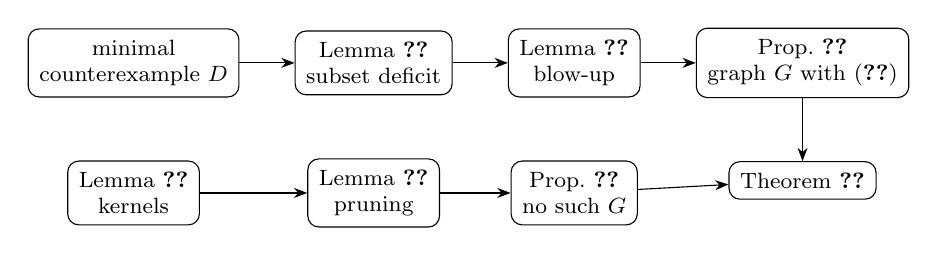
\begin{tikzpicture}[node distance=8mm and 7mm,
  box/.style={draw,rounded corners,align=center,font=\footnotesize,inner sep=4pt}]
 \node[box] (ce) {minimal\\counterexample $D$};
 \node[box,right=of ce] (sd) {Lemma~\ref{lem:subset-deficit}\\subset deficit};
 \node[box,right=of sd] (bl) {Lemma~\ref{lem:blowup}\\blow-up};
 \node[box,right=of bl] (pr) {Prop.~\ref{prop:counterexample-reduction}\\graph $G$ with \eqref{eq:overview-concavity}};
 \node[box,below=of ce] (ks) {Lemma~\ref{lem:kernel-support}\\kernels};
 \node[box,below=of sd] (pl) {Lemma~\ref{lem:pruning}\\pruning};
 \node[box,below=of bl] (nc) {Prop.~\ref{prop:no-concavity}\\no such $G$};
 \node[box,below=of pr] (th) {Theorem~\ref{thm:main}};
 \draw[-{Stealth}] (ce) -- (sd);
 \draw[-{Stealth}] (sd) -- (bl);
 \draw[-{Stealth}] (bl) -- (pr);
 \draw[-{Stealth}] (pr) -- (th);
 \draw[-{Stealth}] (ks) -- (pl);
 \draw[-{Stealth}] (pl) -- (nc);
 \draw[-{Stealth}] (nc) -- (th);
\end{tikzpicture}
\end{center}
Sections~\ref{sec:reduction} and~\ref{sec:pruning} are independent of each
other. Section~\ref{sec:incompatibility} uses only the statements of
Proposition~\ref{prop:counterexample-reduction} and
Lemma~\ref{lem:pruning}.

\subsection{Conventions and renamed symbols}

$\sqcup$ denotes a disjoint union and $\subsetneq$ a proper subset. Vectors
are bold; for a finite set $\mathcal I$, $\R^{\mathcal I}$ is the space of
real vectors indexed by $\mathcal I$, with standard basis $(\be_x)$ and
coordinates $u_x$ of $\bu$. A matrix $\R^{\mathcal J}\to\R^{\mathcal I}$ has
rows indexed by $\mathcal I$ and columns by $\mathcal J$.

The source manuscript reuses several letters. To give each symbol one meaning
they are renamed as follows; the mathematics is unchanged.
In Lemma~\ref{lem:subset-deficit}: $Q,C,d_1,d_2$ become
$Y,\Psi,\nu_1,\nu_2$. In Lemma~\ref{lem:blowup}: $T_v,H_0$ become
$U_v,S^{*}$. In Section~\ref{sec:pruning}: the matrices $D,D^{p,i}$, supports
$T,T^{p,i}$ and index sets $I,J,S_i$ become
$W,W^{p,i},\Theta,\Theta^{p,i},\mathcal I,\mathcal J,\Sigma_i$; the matchings
$\alpha,\beta$ and their endpoint sets $R_\alpha,C_\beta$ become
$\cM_{\cR},\cM_{\cC},\cR_1,\cC_1$; the reached sets $W_L,W_R$ become
$\cV_L^{\star},\cV_R^{\star}$. In Section~\ref{sec:incompatibility} the
abbreviation $M=\abs P+\abs Q$ is written out. In the corollaries,
$A(D),M_D,d^{\pm},Z(v),r$ become
$\Arc(D),\Pi_D,\deg^{\pm},\Non(v),\varrho$.

\section{From a counterexample to a strict subset inequality}
\label{sec:reduction}

Throughout this section $F=F_D$ is the image operator of the base graph $D$
under discussion, and $F_G$ that of the blown-up graph $G$.

\begin{proposition}[Counterexample reduction]
\label{prop:counterexample-reduction}
If Theorem~\ref{thm:main} has a counterexample, then there is a finite
nonempty oriented graph $G$ in which every vertex has positive indegree
and
\begin{equation}
\label{eq:strict-subset-growth}
  \abs{U}+\abs{F_G^2(U)}<2\abs{F_G(U)}
  \qquad\text{for every }\varnothing\ne U\subsetneq V(G).
\end{equation}
\end{proposition}

The proof, at the end of the section, combines
Lemmas~\ref{lem:subset-deficit} and~\ref{lem:blowup}.

\paragraph{Context (not used in the proofs).}
The arc-deletion argument below adapts the proof idea of
\cite[Lemma~4]{Seacrest2019}. Specializing Seacrest's parameter $\lambda$
to $1$, his statement gives
$\abs{F^2(S)\setminus F(S)}<\abs{F(S)}$ in an edge-minimal
counterexample when $F(S)$ is nonempty. Lemma~\ref{lem:subset-deficit}
replaces this right-hand bound by the smaller quantity
$\abs{F(S)\setminus S}$ for nonempty proper $S$, under the stronger choice of
minimum order and then minimum arc count. The comparison is for orientation
only: Seacrest's lemma is not invoked, and
Lemma~\ref{lem:subset-deficit} is proved in full here.

\begin{lemma}[Subset deficit]
\label{lem:subset-deficit}
Suppose that counterexamples exist, that is, nonempty finite oriented graphs
with $\abs{N_1^+(v)}>\abs{N_2^+(v)}$ for every vertex $v$. Let $D$ be a
counterexample with the minimum number of vertices and, among the
counterexamples with that number of vertices, the minimum number of arcs.
Then $D$ is strongly connected, every vertex of $D$ has positive indegree, and
\begin{equation}
\label{eq:subset-deficit}
  \abs{F^2(S)\setminus F(S)}<\abs{F(S)\setminus S}
  \qquad\text{for every }\varnothing\ne S\subsetneq V(D).
\end{equation}
\end{lemma}

\emph{Where it is used:} as the hypothesis of Lemma~\ref{lem:blowup}.

\emph{Plan of the proof.} After three easy consequences of minimality, we
fix $S$, split $F(S)$ into the part $I$ inside $S$ and the part $E$ outside,
and introduce a function $g$ on subsets of $E$ with
$g(\varnothing)=0$ and $g(E)=\abs{F^2(S)\setminus F(S)}$. The core is an
\emph{increment claim}: any $T\subsetneq E$ can be enlarged by a nonempty
set $Y\subseteq E\setminus T$ with $g(T\cup Y)-g(T)<\abs Y$. Growing $T$
from $\varnothing$ to $E$ and adding up gives $g(E)<\abs E$.

\begin{proof}
\Step{Step 1: $D$ has no sink and at least two vertices.}
A sink $v$ has $\abs{N_1^+(v)}=\abs{N_2^+(v)}=0$, so it violates the strict
inequality $\abs{N_1^+(v)}>\abs{N_2^+(v)}$ that every vertex of a
counterexample satisfies. Hence $D$ has no sink; since there are no loops,
$D$ has at least two vertices.

\Step{Step 2: $D$ is strongly connected.}
The strong components of $D$, ordered by reachability, form an acyclic
digraph, so there is a strong component with vertex set $V_0$ such that no
arc leaves $V_0$. For $v\in V_0$ every arc from $v$ ends in $V_0$, and so
does every two-step path from $v$. Therefore $N_1^+(v)$ and $N_2^+(v)$ are
the same in $D$ and in the induced subgraph $D[V_0]$, and $D[V_0]$ is a
counterexample. By minimality of the order, $V_0=V(D)$.

\Step{Step 3: every vertex has an in-neighbour.}
Given $v$, pick a vertex $x\ne v$ (Step~1). By Step~2 there is a directed
path from $x$ to $v$; its last arc enters $v$.

\Step{Step 4: set-up for a fixed $S$.}
Fix $\varnothing\ne S\subsetneq V(D)$ and put
\[
  I=F(S)\cap S,\qquad E=F(S)\setminus S,
  \qquad g(T)=\abs{F(T)\setminus(I\cup T)}\quad(T\subseteq E).
\]
Thus $F(S)=I\sqcup E$, $I\subseteq S$ and $E\cap S=\varnothing$. Moreover
$E\ne\varnothing$: take $x\in S$ and $y\notin S$; a directed path from $x$
to $y$ (Step~2) contains an arc from $S$ to the complement of $S$, and its
head lies in $E$.

\Step{Step 5: increment claim.}
\emph{For every $T\subsetneq E$ there is a nonempty set
$Y\subseteq E\setminus T$ such that}
\begin{equation}
\label{eq:deficit-increment}
  g(T\cup Y)-g(T)<\abs{Y}.
\end{equation}
The set $Y$, and the vertex $v$ used to define it, depend on $T$. Fix
$T\subsetneq E$.

\smallskip\noindent\emph{(5a) The graph $D_T$ and the vertex $v$.}
Let $D_T$ be obtained from the original graph $D$ by deleting all arcs
$x\to y$ with $x\in S$ and $y\in E\setminus T$. Since
$E\setminus T\ne\varnothing$ and every vertex of $E\subseteq F(S)$ is the
head of an arc from $S$, at least one arc is deleted. So $D_T$ is an
oriented graph on the same vertex set with fewer arcs, and by the choice of
$D$ it is not a counterexample. Writing $\tN_1,\tN_2,\tF$ for
$N_1^+,N_2^+,F$ computed in $D_T$, there is a vertex $v$ with
\begin{equation}\label{eq:witness}
 \abs{\tN_1(v)}\le\abs{\tN_2(v)}.
\end{equation}
Since every arc and every path of $D_T$ is also one of $D$, we have
$\tN_1(x)\subseteq N_1^+(x)$ and $\tF^2(\{x\})\subseteq F^2(\{x\})$ for
every vertex $x$.

\smallskip\noindent\emph{(5b) The vertex $v$ lies in $S$ and loses an
out-neighbour.} Suppose $\tN_1(v)=N_1^+(v)$. Then, by
\eqref{eq:exact-second} in $D_T$ and in $D$,
\[
 \tN_2(v)=\tF^2(\{v\})\setminus\tN_1(v)
 \subseteq F^2(\{v\})\setminus N_1^+(v)=N_2^+(v),
\]
so $\abs{N_1^+(v)}=\abs{\tN_1(v)}\le\abs{\tN_2(v)}\le\abs{N_2^+(v)}$,
contradicting that $D$ is a counterexample. Hence some arc leaving $v$ was
deleted. Deleted arcs start in $S$ and end in $E\setminus T$, so
$v\in S$ and
\[
  Y:=N_1^+(v)\cap(E\setminus T)\ne\varnothing,
  \qquad \tN_1(v)=N_1^+(v)\setminus Y .
\]

\smallskip\noindent\emph{(5c) Location of the out-neighbours.}
As $v\in S$, $N_1^+(v)\subseteq F(S)=I\cup T\cup(E\setminus T)$, hence
\[
 N_1^+(v)\subseteq I\cup T\cup Y,\qquad
 \tN_1(v)\subseteq I\cup T,\qquad
 Y\cap(I\cup T)=\varnothing .
\]
The last relation holds because $Y\subseteq E\setminus T$ and
$I\cap E=\varnothing$.

\smallskip\noindent\emph{(5d) Endpoints of two-step paths in $D_T$.}
We claim
\begin{equation}
\label{eq:deleted-path-endpoints}
  \tF^2(\{v\})\subseteq I\cup T\cup F(T).
\end{equation}
Let $v\to u\to w$ be a path in $D_T$. By (5c), $u\in I\cup T$.
If $u\in I\subseteq S$, then in $D$ all arcs from $u$ end in
$F(S)=I\cup T\cup(E\setminus T)$, and those ending in $E\setminus T$ were
deleted; so $w\in I\cup T$. If $u\in T$, then $w\in F(T)$.

\smallskip\noindent\emph{(5e) Gained second out-neighbours:
$\tN_2(v)\setminus N_2^+(v)\subseteq Y\cap F(T)$.}
Let $w\in\tN_2(v)\setminus N_2^+(v)$. Then
$w\in\tF^2(\{v\})\subseteq F^2(\{v\})$. Since
$w\notin N_2^+(v)=F^2(\{v\})\setminus N_1^+(v)$, necessarily
$w\in N_1^+(v)$. Since $w\in\tN_2(v)$, we have
$w\notin\tN_1(v)=N_1^+(v)\setminus Y$. Hence $w\in Y$. Finally
$w\in I\cup T\cup F(T)$ by \eqref{eq:deleted-path-endpoints} and
$w\notin I\cup T$ by (5c), so $w\in F(T)$.

\smallskip\noindent\emph{(5f) Lost second out-neighbours.} Define
\[
  \Psi=F(Y)\setminus\bigl(I\cup T\cup Y\cup F(T)\bigr).
\]
Then $\Psi\subseteq N_2^+(v)\setminus\tN_2(v)$. Indeed, let $w\in\Psi$.
There is $y\in Y\subseteq N_1^+(v)$ with $y\to w$, so $w\in F^2(\{v\})$;
and $w\notin I\cup T\cup Y\supseteq N_1^+(v)$ by (5c). So
$w\in N_2^+(v)$ by \eqref{eq:exact-second}. (Orientedness enters here
through \eqref{eq:exact-second}: $w\ne v$ because an arc $y\to v$ would
oppose $v\to y$.) On the other hand $w\notin I\cup T\cup F(T)$, so
$w\notin\tF^2(\{v\})\supseteq\tN_2(v)$ by
\eqref{eq:deleted-path-endpoints}.

\smallskip\noindent\emph{(5g) Counting.}
By (5e) and (5f), a vertex of $\tN_2(v)$ either lies in $N_2^+(v)$, and
then not in $\Psi$, or lies in $Y\cap F(T)$:
\[
 \tN_2(v)\subseteq\bigl(N_2^+(v)\setminus\Psi\bigr)\cup\bigl(Y\cap F(T)\bigr).
\]
Write $\nu_1=\abs{N_1^+(v)}$ and $\nu_2=\abs{N_2^+(v)}$, so
$\nu_2<\nu_1$. Using (5b), \eqref{eq:witness}, and
$\Psi\subseteq N_2^+(v)$,
\begin{equation}\label{eq:gain-loss}
  \nu_1-\abs{Y}=\abs{\tN_1(v)}
  \le \abs{\tN_2(v)}
  \le \nu_2-\abs{\Psi}+\abs{Y\cap F(T)}.
\end{equation}

\smallskip\noindent\emph{(5h) The change in $g$ is exactly
$\abs\Psi-\abs{Y\cap F(T)}$.}
Put $\Omega=F(T)\setminus(I\cup T\cup Y)$. Since
$Y\cap(I\cup T)=\varnothing$,
\[
 F(T)\setminus(I\cup T)=\Omega\sqcup\bigl(F(T)\cap Y\bigr),
 \qquad\text{so}\qquad g(T)=\abs\Omega+\abs{Y\cap F(T)}.
\]
Since $F(T\cup Y)=F(T)\cup F(Y)$, and the part of
$F(Y)\setminus(I\cup T\cup Y)$ outside $F(T)$ is by definition $\Psi$,
\[
 F(T\cup Y)\setminus(I\cup T\cup Y)=\Omega\sqcup\Psi,
 \qquad\text{so}\qquad g(T\cup Y)=\abs\Omega+\abs\Psi .
\]

\smallskip\noindent\emph{(5i) Conclusion of the claim.}
By (5h), then \eqref{eq:gain-loss} rearranged, then $\nu_2<\nu_1$,
\[
  g(T\cup Y)-g(T)
  =\abs{\Psi}-\abs{Y\cap F(T)}
  \le \abs{Y}+\nu_2-\nu_1
  <\abs{Y}.
\]

\Step{Step 6: summing the increments.}
Set $T_0=\varnothing$. As long as $T_k\ne E$, apply Step~5 to $T=T_k$
(each time deleting arcs from the \emph{original} graph $D$, so that
Step~5 applies verbatim), obtain a nonempty $Y_k\subseteq E\setminus T_k$,
and set $T_{k+1}=T_k\sqcup Y_k$. The sets $Y_k$ are nonempty and pairwise
disjoint subsets of the finite set $E$, so the process stops at some
$T_r=E$ with $r\ge1$ (as $E\ne\varnothing$), and
$\sum_{k<r}\abs{Y_k}=\abs E$. Telescoping~\eqref{eq:deficit-increment},
\[
 g(E)-g(\varnothing)=\sum_{k<r}\bigl(g(T_{k+1})-g(T_k)\bigr)
 <\sum_{k<r}\abs{Y_k}=\abs E .
\]
Also $g(\varnothing)=\abs{F(\varnothing)\setminus I}=0$. Hence
$g(E)<\abs E$.

\Step{Step 7: identification of $g(E)$.}
Since $F(S)=I\cup E$ we have $F^2(S)=F(I)\cup F(E)$, and
$F(I)\subseteq F(S)$ because $I\subseteq S$. Therefore
\[
  F^2(S)\setminus F(S)
  =\bigl(F(I)\cup F(E)\bigr)\setminus(I\cup E)
  =F(E)\setminus(I\cup E),
\]
whose cardinality is $g(E)$. With Step~6 and $\abs E=\abs{F(S)\setminus S}$
this is \eqref{eq:subset-deficit}.
\end{proof}

We next amplify the integer deficit in \eqref{eq:subset-deficit}.
Each unit of the base deficit contributes the entire block size; the
remaining internal contribution costs at most one unit per base vertex.
The construction is the lexicographic product of $D$ with a transitive
tournament. The same graph-product construction appears
in \cite[Theorem~4.3]{BrantnerBrockmanKaySnively2009}; here we need an
estimate for every nonempty proper subset, rather than only for individual
vertices.

\begin{lemma}[Transitive-tournament blowup]
\label{lem:blowup}
Let $D$ be an oriented graph on $n\ge1$ vertices, all of positive
indegree, satisfying \eqref{eq:subset-deficit} for every nonempty proper
subset of $V(D)$. For an integer $m>n$, replace each vertex by a
transitive tournament on $m$ vertices. For every arc $v\to w$ of $D$,
put all arcs from the block at $v$ to the block at $w$, and put no other
arcs between distinct blocks. The resulting graph $G$ is oriented,
all its indegrees are positive, and it satisfies
\eqref{eq:strict-subset-growth}.
\end{lemma}

\emph{Where it is used:} in the proof of
Proposition~\ref{prop:counterexample-reduction}.

\emph{Plan of the proof.} For $U\subseteq V(G)$ let $S$ be the set of
blocks that $U$ meets. We compute $\abs{F_G(U)}$ exactly and bound
$\abs{F_G^2(U)}$ from above, block by block. Full blocks contribute
multiples of $m$ governed by the deficit of $S$ in $D$; partial blocks
contribute at most $1$ each. The case $S=V(D)$ is treated separately.

\begin{proof}
Explicitly, $V(G)=V(D)\times\{1,\dots,m\}$, and $(v,a)\to(w,b)$ if and only
if either $v=w$ and $a<b$ (an \emph{internal} arc), or $v\to w$ in $D$ (an
\emph{external} arc). The \emph{block} of $v$ is $\{v\}\times\{1,\dots,m\}$.

\Step{Step 1: the internal image operator.}
For a set $\Lambda\subseteq\{1,\dots,m\}$ of labels let
$f(\Lambda)=\{b:a<b\text{ for some }a\in\Lambda\}$. Thus
$f(\varnothing)=\varnothing$ and
$f(\Lambda)=\{\min\Lambda+1,\dots,m\}$ for $\Lambda\ne\varnothing$. For
nonempty $\Lambda$ we have $\abs\Lambda\le m-\min\Lambda+1=\abs{f(\Lambda)}+1$
and $f^2(\Lambda)=f(f(\Lambda))\subseteq f(\Lambda)$, hence
\begin{equation}
\label{eq:internal-block-bound}
  \abs{\Lambda}-\abs{f(\Lambda)}\le1,\qquad
  \abs{f^2(\Lambda)}\le\abs{f(\Lambda)},\qquad
  \abs{\Lambda}-2\abs{f(\Lambda)}+\abs{f^2(\Lambda)}\le1 .
\end{equation}

\Step{Step 2: $G$ is oriented with positive indegrees.}
There are no loops. Two opposite internal arcs would need $a<b$ and $b<a$;
two opposite external arcs would project to opposite arcs of $D$; an
internal and an external arc never join the same pair of vertices. Every
vertex $(w,b)$ receives an arc from $(v,1)$, where $v$ is an in-neighbour
of $w$ in $D$.

\Step{Step 3: notation for a fixed $U$.}
Fix $\varnothing\ne U\subsetneq V(G)$. For $v\in V(D)$ let
$U_v=\{a:(v,a)\in U\}$, and put
\[
  S=\{v\in V(D):U_v\ne\varnothing\},\qquad
  S^{*}=F(S)\cup F^2(S).
\]
Then $S\ne\varnothing$ and $\abs U=\sum_{v\in S}\abs{U_v}$.

\Step{Step 4: the first image, exactly.}
Let $w\in V(D)$. If $w\in F(S)$, choose $v\in S$ with $v\to w$ and
$(v,a)\in U$; then $(v,a)$ sends an arc to every vertex of the block of
$w$, so the whole block lies in $F_G(U)$. If $w\notin F(S)$, no external
arc from $U$ enters the block of $w$, so $F_G(U)$ meets this block exactly
in $\{w\}\times f(U_w)$; this is empty when $w\notin S$. Hence
\begin{equation}\label{eq:first-image}
  \abs{F_G(U)}=m\abs{F(S)}
     +\sum_{v\in S\setminus F(S)}\abs{f(U_v)}.
\end{equation}

\Step{Step 5: the second image, from above.}
We claim
\begin{equation}\label{eq:second-image}
  \abs{F_G^2(U)}\le m\abs{S^{*}}
     +\sum_{v\in S\setminus S^{*}}\abs{f^2(U_v)}.
\end{equation}
Blocks of vertices in $S^{*}$ contribute at most $m$ each. Let
$w\notin S^{*}$ and let $y\in F_G^2(U)$ lie in the block of $w$; choose
$x\in U$ and $z$ with $x\to z\to y$, and let $v\in S$ and $u$ be the base
vertices of $x$ and $z$.
\begin{itemize}[leftmargin=2em]
\item If $x\to z$ is external, then $u\in F(S)$. If $z\to y$ is external
then $w\in F(\{u\})\subseteq F^2(S)$; if internal then $w=u\in F(S)$. Both
contradict $w\notin S^{*}$.
\item If $x\to z$ is internal, then $u=v$. If $z\to y$ is external then
$w\in F(\{v\})\subseteq F(S)$, again impossible. So both arcs are internal,
$w=v\in S\setminus S^{*}$, and the label of $y$ lies in $f^2(U_v)$.
\end{itemize}
This proves \eqref{eq:second-image}.

\Step{Step 6: combining.}
From Step~3, \eqref{eq:first-image} and \eqref{eq:second-image},
\begin{align}
\label{eq:blowup-sharp}
  \abs{U}-2\abs{F_G(U)}+\abs{F_G^2(U)}
  &\le m\bigl(\abs{S^{*}}-2\abs{F(S)}\bigr)
       +\sum_{v\in S}\abs{U_v} \notag\\
  &\quad -2\sum_{v\in S\setminus F(S)}\abs{f(U_v)}
       +\sum_{v\in S\setminus S^{*}}\abs{f^2(U_v)}.
\end{align}
Since $F(S)\subseteq S^{*}$, we have
$S\setminus S^{*}\subseteq S\setminus F(S)$, and enlarging the last sum to
$S\setminus F(S)$ only adds nonnegative terms. Now split
$\sum_{v\in S}\abs{U_v}$ over $S\cap F(S)$ and $S\setminus F(S)$; use
$\abs{U_v}\le m$ on $S\cap F(S)$ and the third inequality of
\eqref{eq:internal-block-bound} (valid because $U_v\ne\varnothing$) on
$S\setminus F(S)$:
\begin{align*}
  \abs{U}-2\abs{F_G(U)}+\abs{F_G^2(U)}
  &\le m\bigl(\abs{S^{*}}-2\abs{F(S)}
                    +\abs{S\cap F(S)}\bigr)
       +\abs{S\setminus F(S)}\\
  &\le m\bigl(\abs{F^2(S)\setminus F(S)}
                    -\abs{F(S)\setminus S}\bigr)+n.
\end{align*}
The last line uses $\abs{S^{*}}=\abs{F(S)}+\abs{F^2(S)\setminus F(S)}$,
$\abs{F(S)}-\abs{S\cap F(S)}=\abs{F(S)\setminus S}$, and
$\abs{S\setminus F(S)}\le n$.

\Step{Step 7: the case $S\subsetneq V(D)$.}
Then $S$ is nonempty and proper, so by \eqref{eq:subset-deficit} the
parenthesized difference is an integer $\le-1$. The bound of Step~6 is at
most $-m+n<0$, which is \eqref{eq:strict-subset-growth}.

\Step{Step 8: the case $S=V(D)$.}
Here \eqref{eq:subset-deficit} is not available. Positive indegrees in $D$
give $F(S)=V(D)$, so $F_G(U)=V(G)$ by Step~4. Positive indegrees in $G$
(Step~2) give $F_G^2(U)=F_G(V(G))=V(G)$. Hence
\[
  \abs{U}-2\abs{F_G(U)}+\abs{F_G^2(U)}
  =\abs{U}-\abs{V(G)}<0,
\]
because $U$ is proper.
\end{proof}

\begin{proof}[Proof of Proposition~\ref{prop:counterexample-reduction}]
Choose a counterexample $D$ of minimum order and then minimum number of
arcs. Lemma~\ref{lem:subset-deficit} supplies positive indegrees and
the subset deficit \eqref{eq:subset-deficit}, so Lemma~\ref{lem:blowup},
with any integer $m>\abs{V(D)}$, supplies the required graph $G$.
\end{proof}

\section{Pruning two families of pairs}\label{sec:pruning}

This section is independent of Section~\ref{sec:reduction} and involves no
graph: only a finite set with a binary relation. The bound proved here
charges the deleted members to two sets of pairs: one determined by the
original conflicts, and the other consisting of points left uncovered after
deletion.

\begin{lemma}[Pruning]\label{lem:pruning}
Let $X$ be a finite set with a binary relation denoted by $\to$, and let
$\mathcal R,\mathcal C\subseteq X\times X$ be two families, regarded as
separate copies even when their coordinates agree. Say that
$(p,j)\in\mathcal R$ and $(i,s)\in\mathcal C$ \emph{conflict} if
\[
 p\to i\qquad\text{and}\qquad s\to j.
\]
Define
\begin{align*}
 Z&=\{(i,j):\text{some }(p,j)\in\mathcal R
       \text{ conflicts with some }(i,s)\in\mathcal C\},\\
 H&=\{(p,s):\text{some }(p,j)\in\mathcal R
       \text{ conflicts with some }(i,s)\in\mathcal C\}.
\end{align*}
A point $(i,j)$ is \emph{covered} by a member $(p,j)\in\mathcal R$ when
$p\to i$, and by a member $(i,s)\in\mathcal C$ when $s\to j$.
These are the only ways a member covers a point.

There are subfamilies $\mathcal R'\subseteq\mathcal R$ and
$\mathcal C'\subseteq\mathcal C$ with no conflicts between them such that
every initially conflict-free member is retained and
\begin{equation}\label{eq:pruning-bound}
 \abs{\mathcal R\setminus\mathcal R'}+
 \abs{\mathcal C\setminus\mathcal C'}
 \leq \abs H+
 \abs{\{z\in Z:z\text{ is covered by no member of }
                    \mathcal R'\cup\mathcal C'\}}.
\end{equation}
The two sides are counted separately throughout.
\end{lemma}

\emph{Reading the statement.} ``Counted separately'' means that a pair lying
in both $\cR$ and $\cC$ is two members, one on each side; the left-hand side
of \eqref{eq:pruning-bound} counts deletions on each side separately.
A member is \emph{initially conflict-free} if it conflicts with no member of
the other family. In a conflict the four elements $p,i,s,j$ give the two
members $(p,j),(i,s)$ and two further pairs: $(i,j)\in Z$, obtained from
$(p,j)$ by advancing the first coordinate along $p\to i$, and
$(p,s)\in H$, obtained from $(p,j)$ by moving the second coordinate back
along $s\to j$.

\emph{Where it is used:} once, in Step~8 of the proof of
Proposition~\ref{prop:no-concavity}.

\begin{remark}[The lemma is existential, and the last term is needed]
Let $X=\{p,s,i_1,i_2,j_1,j_2\}$ with $p\to i_1$, $p\to i_2$, $s\to j_1$,
$s\to j_2$, and let $\cR=\{(p,j_1),(p,j_2)\}$,
$\cC=\{(i_1,s),(i_2,s)\}$. Every member of $\cR$ conflicts with every member
of $\cC$, $H=\{(p,s)\}$ and $Z=\{i_1,i_2\}\times\{j_1,j_2\}$. A conflict-free
pair must delete one family entirely. Deleting only $\cC$ costs $2$ and
leaves every point of $Z$ covered, so it violates \eqref{eq:pruning-bound}
(the right side is $1$); deleting everything costs $4\le 1+4$. So a
cheapest pruning need not satisfy the bound, and the bound $\abs H$ alone
would be false.
\end{remark}

We first record the elementary rank fact used in the proof. A real matrix
\emph{supported on} a set $\Theta$ of positions is one whose entries outside
$\Theta$ are zero; entries in $\Theta$ are allowed to vanish.

\begin{lemma}[Kernels at maximum support rank]\label{lem:kernel-support}
Let $\mathcal I,\mathcal J$ be finite sets and
$\Theta\subseteq\mathcal I\times\mathcal J$. Suppose that
$W:\R^{\mathcal J}\to\R^{\mathcal I}$ has maximum rank among all real
matrices supported on $\Theta$.
Then, for every $\bx\in\ker W$, every $\by\in\ker W\tp$, and every
$(s,j)\in\Theta$, one has $x_jy_s=0$.
\end{lemma}

\emph{Where it is used:} in Part~8 of the proof of
Lemma~\ref{lem:pruning}, applied to fixed real matrices $W^{p,i}$.

\begin{proof}
Suppose $x_jy_s\ne0$ for some $(s,j)\in\Theta$. Let
$W_1=W+\be_s\be_j\tp$, the matrix $W$ with $1$ added to its $(s,j)$ entry.
It is supported on $\Theta$.
\begin{enumerate}[label=(\arabic*),leftmargin=2em]
\item $W_1\bx=W\bx+x_j\be_s=x_j\be_s$ and $x_j\ne0$, so
$\be_s\in\im W_1$.
\item For every $\mathbf w\in\R^{\mathcal J}$,
$W\mathbf w=W_1\mathbf w-w_j\be_s\in\im W_1$ by (1). So
$\im W\subseteq\im W_1$.
\item $\by\tp W=0$, so $\by$ is orthogonal to $\im W$; but
$\by\tp\be_s=y_s\ne0$. So $\be_s\notin\im W$.
\end{enumerate}
By (1)--(3), $\im W_1\supseteq\im W+\R\be_s\supsetneq\im W$, so
$\rank W_1>\rank W$, contradicting maximality.
\end{proof}

\begin{proof}[Proof of Lemma~\ref{lem:pruning}]
\emph{Plan.} Parts~1--2 reduce the lemma to finding a small vertex cover in
a bipartite graph $\Gamma$. Parts~3--9 show that a maximum matching of
$\Gamma$ has at most $\abs Z+\abs H$ edges. Part~10 converts the matching
bound into the cover (K\H{o}nig's theorem, proved here).

\Step{Part 0: trivial case and conventions.}
If there are no conflicts, retain every member; then
$Z=H=\varnothing$ and \eqref{eq:pruning-bound} reads $0\le0$. Assume there is
at least one conflict. A $0\times0$ minor has determinant $1$, so the rank
arguments below also apply when a matching or an index set is empty.

\Step{Part 1: the augmented bipartite graph $\Gamma$.}
Let $Z_L$ and $Z_R$ be two disjoint copies of $Z$, disjoint from $\cR$ and
$\cC$; write $z_L,z_R$ for the copies of $z\in Z$. Let $\Gamma$ be the
bipartite graph with parts
\[
 \mathcal V_L=\mathcal R\sqcup Z_L,
 \qquad
 \mathcal V_R=\mathcal C\sqcup Z_R,
\]
and the following edges:
\begin{itemize}[leftmargin=2em]
\item $\{r,c\}$ for $r\in\cR$, $c\in\cC$ that conflict;
\item $\{r,z_R\}$ for $r\in\cR$ and $z\in Z$ covered by $r$;
\item $\{z_L,c\}$ for $c\in\cC$ and $z\in Z$ covered by $c$.
\end{itemize}
There are no edges between $Z_L$ and $Z_R$. We call the members of
$\cR\sqcup\cC$ \emph{original} vertices.
Figure~\ref{fig:pruning} displays the three edges forced by one conflict.

\begin{figure}[!ht]
 \centering
 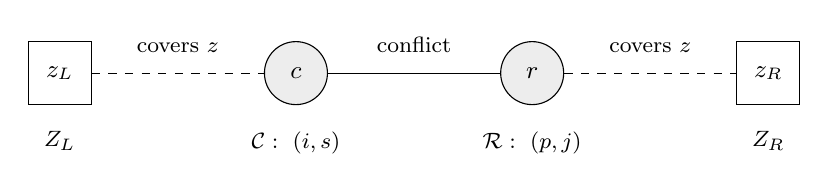
\begin{tikzpicture}[
  every node/.style={font=\small},
  original/.style={circle,draw,fill=black!7,minimum size=8mm,inner sep=1pt},
  copy/.style={rectangle,draw,minimum size=8mm,inner sep=3pt},
  edge label/.style={font=\footnotesize,above=4pt},
  family label/.style={font=\footnotesize,below=6pt}
]
 \node[copy] (zl) at (0,0) {$z_L$};
 \node[original] (c) at (3,0) {$c$};
 \node[original] (r) at (6,0) {$r$};
 \node[copy] (zr) at (9,0) {$z_R$};
 \draw[dashed] (zl) -- node[edge label] {covers $z$} (c);
 \draw (c) -- node[edge label] {conflict} (r);
 \draw[dashed] (r) -- node[edge label] {covers $z$} (zr);
 \node[family label] at (zl.south) {$Z_L$};
 \node[family label] at (c.south) {$\mathcal C:\ (i,s)$};
 \node[family label] at (r.south) {$\mathcal R:\ (p,j)$};
 \node[family label] at (zr.south) {$Z_R$};
\end{tikzpicture}

 \caption{A conflict between $r=(p,j)$ and $c=(i,s)$ forces this path,
 where $z=(i,j)\in Z$. The copies $z_L$ and $z_R$ are distinct vertices.
 The vertices alternate between the two sides of the bipartition.
 Different conflicts can share vertices and edges; the full augmented
 graph need not be a disjoint union of such paths.}
 \label{fig:pruning}
\end{figure}

\emph{Claim 1: an initially conflict-free member is isolated in $\Gamma$.}
It has no conflict edge by definition. Suppose $(p,j)\in\cR$ covers
$(i,j)\in Z$, so $p\to i$. Since $(i,j)\in Z$, some
$(p',j)\in\cR$ conflicts with some $(i,s)\in\cC$; in particular $s\to j$.
Then $p\to i$ and $s\to j$, so $(p,j)$ conflicts with $(i,s)$. Symmetrically,
if $(i,s)\in\cC$ covers $(i,j)\in Z$, so $s\to j$, a witness
$(p,j)\in\cR$, $(i,s')\in\cC$ of $(i,j)\in Z$ has $p\to i$, and $(p,j)$
conflicts with $(i,s)$. So a member with a cover edge is not conflict-free.

\Step{Part 2: a small vertex cover suffices.}
\emph{Claim 2: if $K$ is a vertex cover of $\Gamma$ with
$\abs K\le\abs Z+\abs H$ that contains no isolated vertex, then
$\cR'=\cR\setminus K$ and $\cC'=\cC\setminus K$ satisfy the lemma.}

No conflict survives, because every conflict edge has an endpoint in $K$.
Conflict-free members are isolated (Claim~1), hence not in $K$, hence
retained. Let $q$ be the number of points of $Z$ covered by no member of
$\cR'\cup\cC'$. Each of the other $\abs Z-q$ points $z$ is covered by a
surviving member, which is adjacent to $z_R$ (if it is in $\cR'$) or to
$z_L$ (if it is in $\cC'$). That edge must be covered by $K$, and the
surviving member is not in $K$, so the copy of $z$ is in $K$. Distinct
points have distinct copies, so
$\abs{K\cap(Z_L\sqcup Z_R)}\ge\abs Z-q$ and
\begin{equation}\label{eq:cover-charge}
 \abs{\cR\setminus\cR'}+\abs{\cC\setminus\cC'}
 =\abs{K\cap(\mathcal R\sqcup\mathcal C)}
 \leq \abs K-(\abs Z-q)\leq\abs H+q .
\end{equation}
This is \eqref{eq:pruning-bound}.

\Step{Part 3: a maximum matching and its three parts.}
Among all maximum matchings of $\Gamma$ choose one, $\cM$, with the fewest
edges joining two original vertices. Split
$\cM=\cM_0\sqcup\cM_{\cR}\sqcup\cM_{\cC}$ into its edges between $\cR$ and
$\cC$, between $\cR$ and $Z_R$, and between $Z_L$ and $\cC$, and put
\[
 k=\abs{\cM_0},\qquad\ell=\abs{\cM_{\cR}},\qquad t=\abs{\cM_{\cC}},
 \qquad\abs{\mathcal M}=k+\ell+t.
\]
Let $\cR_0,\cR_1\subseteq\cR$ be the sets of members of $\cR$ matched by
$\cM_0$ and by $\cM_{\cR}$, and $\cC_0,\cC_1\subseteq\cC$ those matched by
$\cM_0$ and by $\cM_{\cC}$. As $\cM$ is a matching,
$\cR_0\cap\cR_1=\varnothing=\cC_0\cap\cC_1$, and
$\abs{\cR_0}=k$, $\abs{\cR_1}=\ell$, $\abs{\cC_1}=t$.
Let $\Gamma_{\cR}$ be the subgraph of $\Gamma$ induced on $\cR\sqcup Z_R$
and $\Gamma_{\cC}$ the one induced on $Z_L\sqcup\cC$.

\emph{Claim 3: $\cM_{\cR}$ is a maximum matching of $\Gamma_{\cR}$, and
$\cM_{\cC}$ is a maximum matching of $\Gamma_{\cC}$.}

We prove the first assertion; the second is the same with the two sides
exchanged. Two facts: (F1) a vertex of $Z_R$ is adjacent only to vertices
of $\cR$, so it is matched by $\cM$ if and only if it is matched by
$\cM_{\cR}$; (F2) a vertex of $\cR$ is adjacent only to vertices of
$\cC\sqcup Z_R$, so if it is matched by $\cM$ but not by $\cM_{\cR}$, it is
matched by $\cM_0$.

Suppose $\Gamma_{\cR}$ has a matching $\cM'$ with more than $\ell$ edges.
In the symmetric difference of $\cM_{\cR}$ and $\cM'$ every vertex has
degree at most $2$, so its components are paths and cycles whose edges
alternate between the two matchings. Some component has more edges of $\cM'$
than of $\cM_{\cR}$; it is a path $\pi$ of odd length whose first and last
edges are in $\cM'$ and whose two end vertices are unmatched by
$\cM_{\cR}$. Being of odd length in a bipartite graph, $\pi$ has one end
$r\in\cR$ and the other end $z_R\in Z_R$. By (F1), $z_R$ is unmatched in
$\cM$. Every internal vertex of $\pi$ is matched in $\cM$ by an edge of
$\cM_{\cR}$ on $\pi$, and the other edges of $\pi$ are not in $\cM$ (they
are edges of $\Gamma_{\cR}$ outside $\cM_{\cR}$).
\begin{itemize}[leftmargin=2em]
\item If $r$ is unmatched in $\cM$, exchanging along $\pi$ (remove the edges
of $\pi$ in $\cM$, add the others) gives a matching of $\Gamma$ with
$\abs\cM+1$ edges, contradicting maximality.
\item Otherwise, by (F2), $r$ lies on an edge $e\in\cM_0$. In
$\cM\setminus\{e\}$ the vertex $r$ is unmatched, so exchanging along $\pi$
gives a matching with $(\abs\cM-1)+1=\abs\cM$ edges whose
original--original edges are $\cM_0\setminus\{e\}$, that is, $k-1$ of them.
This contradicts the choice of $\cM$.
\end{itemize}

\Step{Part 4: four matrices with $NL=AB$.}
For each ordered pair $(x,y)$ with $x\to y$ introduce two variables
$a_{xy}$ and $b_{xy}$, all distinct. For $x\not\to y$ set
$a_{xy}=b_{xy}=0$. For any assignment of real values to the variables,
define four matrices
\[
 \begin{array}{ccc}
 \R^{\mathcal R}&\xrightarrow{\ L\ }&\R^Z\\[3pt]
 {\scriptstyle B}\big\downarrow&&\big\downarrow{\scriptstyle N}\\[3pt]
 \R^H&\xrightarrow{\ A\ }&\R^{\mathcal C}
 \end{array}
\]
with entries
\begin{equation}\label{eq:pruning-maps}
 \begin{aligned}
 L_{(i,j),(p,j)}&=a_{pi},&
 N_{(i,s),(i,j)}&=b_{sj},\\
 B_{(p,s),(p,j)}&=b_{sj},&
 A_{(i,s),(p,s)}&=a_{pi}.
 \end{aligned}
\end{equation}
In each formula the row index is written first and ranges over the target's
index set, the column index over the source's. Every entry not of a listed
form is zero: an entry of $L$ or $A$ vanishes unless row and column have the
\emph{same second coordinate}, and an entry of $N$ or $B$ vanishes unless
they have the \emph{same first coordinate}. So $L,A$ advance the first
coordinate along $p\to i$, and $N,B$ move the second coordinate back from
$j$ to $s$ along $s\to j$. Two consequences of the convention
$a_{xy}=b_{xy}=0$ for $x\not\to y$:
\begin{itemize}[leftmargin=2em]
\item[(O1)] $L_{z,r}\ne0$ only if $r\in\cR$ covers $z$, that is, only if
$\{r,z_R\}$ is an edge of $\Gamma_{\cR}$;
\item[(O2)] $N_{c,z}\ne0$ only if $c\in\cC$ covers $z$, that is, only if
$\{z_L,c\}$ is an edge of $\Gamma_{\cC}$.
\end{itemize}

\emph{Claim 4:} for every assignment,
\begin{equation}\label{eq:pruning-commute}
 NL=AB.
\end{equation}
Fix a column $(p,j)\in\cR$ and a row $(i,s)\in\cC$. In
$(NL)_{(i,s),(p,j)}=\sum_{z\in Z}N_{(i,s),z}L_{z,(p,j)}$ a term can be
nonzero only if $z$ has first coordinate $i$ and second coordinate $j$, so
the sum is $b_{sj}a_{pi}$ if $(i,j)\in Z$ and $0$ otherwise. Likewise
$(AB)_{(i,s),(p,j)}$ is $a_{pi}b_{sj}$ if $(p,s)\in H$ and $0$ otherwise. If
$(p,j)$ and $(i,s)$ conflict, then $(i,j)\in Z$ and $(p,s)\in H$, and both
entries equal $a_{pi}b_{sj}$. If they do not conflict, then $p\not\to i$ or
$s\not\to j$, so $a_{pi}b_{sj}=0$ and both entries are $0$.

\Step{Part 5: three rank conditions imply the matching bound.}
\emph{Claim 5: if for some real assignment}
\begin{equation}\label{eq:three-conditions}
 \rank L=\ell,\qquad \rank N=t,\qquad \dim\ker A\geq k,
\end{equation}
\emph{then $\abs{\cM}=k+\ell+t\le\abs Z+\abs H$.}
Indeed, by rank--nullity for $A:\R^H\to\R^{\cC}$, then
$\rank A\ge\rank(AB)$, then \eqref{eq:pruning-commute},
\begin{align}
 \abs H
 &=\dim\ker A+\rank A
 \geq k+\rank(AB)= k+\rank(NL)
 \geq k+\ell+t-\abs Z.
 \label{eq:pruning-rank-bound}
\end{align}
The last inequality is rank--nullity for $N$ restricted to $\im L$:
\[
 \rank(NL)
 =\dim\im L-\dim(\im L\cap\ker N)
 \geq\ell-\dim\ker N=\ell-(\abs Z-t).
\]
Parts~6--9 produce an assignment satisfying \eqref{eq:three-conditions}.

\Step{Part 6: one assignment satisfying finitely many genericity conditions.}
The correspondence between generic matrix rank and maximum matching size is
due to Edmonds~\cite[Section~5, Theorem~1]{Edmonds1967}; everything needed
is proved here. Let $\R[a,b]$ be the polynomial ring in all the variables
$a_{xy},b_{xy}$ ($x\to y$). It is an integral domain, so a product of
nonzero polynomials is nonzero. The entries of $L$ and $N$, and of the
matrices $W^{p,i}$ defined below, are variables or $0$, so each minor of
these matrices is an element of $\R[a,b]$, and its value at a real
assignment is the corresponding minor of the real matrix.

\smallskip\noindent\emph{(6a) $\rank L\le\ell$ and $\rank N\le t$ for every
real assignment.} Suppose $L$ has a nonzero $h\times h$ minor, with column
set $\cR^{\circ}\subseteq\cR$ and row set $Z^{\circ}\subseteq Z$. Some term
of the Leibniz expansion is nonzero: there is a bijection
$\varphi:\cR^{\circ}\to Z^{\circ}$ with $L_{\varphi(r),r}\ne0$ for all
$r\in\cR^{\circ}$. By (O1) the edges $\{r,\varphi(r)_R\}$ form a matching
of $\Gamma_{\cR}$ with $h$ edges, so $h\le\ell$ by Claim~3. The same
argument with (O2) and $\Gamma_{\cC}$ gives $\rank N\le t$.

\smallskip\noindent\emph{(6b) The matching minor $\pi_L$ of $L$ is a
nonzero polynomial.} Let $Z_{\cR}\subseteq Z$ be the set of points $z$ with
$z_R$ matched by $\cM_{\cR}$, and let $\varphi_0:\cR_1\to Z_{\cR}$ be the
bijection given by $\cM_{\cR}$. Let $\pi_L\in\R[a,b]$ be the determinant of
the $\ell\times\ell$ submatrix of $L$ with columns $\cR_1$ and rows
$Z_{\cR}$. An edge $\{r,z_R\}$ means that $r=(p,j)$ covers $z=(i,j)$: the
second coordinates agree and $p\to i$. So $\varphi_0$ preserves second
coordinates. Group the columns in $\cR_1$ and the rows in $Z_{\cR}$ by
their second coordinate $j$; for each $j$ the two groups have the same size
(via $\varphi_0$), and entries of $L$ between different groups vanish. So
the submatrix is block diagonal up to reordering, and
$\pi_L=\pm\prod_j\pi_{L,j}$, where $\pi_{L,j}$ is the determinant of the
block for $j$.

Fix $j$. The block has columns $(p,j)$, $p\in P^j$, rows $(i,j)$,
$i\in I^j$, and entry $a_{pi}$ in position $((i,j),(p,j))$. Its determinant
is
\[
 \pi_{L,j}=\sum_{\sigma}\pm\prod_{p\in P^j}a_{p\,\sigma(p)},
\]
summed over bijections $\sigma:P^j\to I^j$; the term of $\sigma$ is nonzero
exactly when $p\to\sigma(p)$ for all $p$, and then it is a product of
$\abs{P^j}$ \emph{distinct} variables. This monomial determines $\sigma$:
the variable $a_{pi}$ occurs in it if and only if $\sigma(p)=i$. Hence
different bijections give different monomials and nothing cancels. The
bijection induced by $\varphi_0$ satisfies $p\to\sigma(p)$ for all $p$, so
its monomial occurs with coefficient $\pm1$. Thus $\pi_{L,j}\ne0$ in
$\R[a,b]$. The same variable $a_{pi}$ may occur in blocks for different $j$;
this is why we argue block by block and then use that $\R[a,b]$ is an
integral domain to conclude $\pi_L\ne0$.

\smallskip\noindent\emph{(6c) The matching minor $\pi_N$ of $N$ is a
nonzero polynomial.} Let $Z_{\cC}\subseteq Z$ be the set of points $z$ with
$z_L$ matched by $\cM_{\cC}$, and $\pi_N$ the determinant of the
$t\times t$ submatrix of $N$ with rows $\cC_1$ and columns $Z_{\cC}$. An
edge $\{z_L,c\}$ means that $c=(i,s)$ covers $z=(i,j)$: the first coordinates
agree and $s\to j$. Repeating (6b) with blocks of constant \emph{first}
coordinate $i$, in which the entries are distinct variables $b_{sj}$, gives
$\pi_N\ne0$.

\smallskip\noindent\emph{(6d) The auxiliary matrices $W^{p,i}$.}
For every pair with $p\to i$ define
\[
 J_p=\{j:(p,j)\in\mathcal R\},\qquad
 \Sigma_i=\{s:(i,s)\in\mathcal C\},\qquad
 W^{p,i}=(b_{sj})_{s\in \Sigma_i,\ j\in J_p},
\]
a matrix $\R^{J_p}\to\R^{\Sigma_i}$, and
\[
 \Theta^{p,i}=\{(s,j)\in \Sigma_i\times J_p:s\to j\}.
\]
The entries of $W^{p,i}$ in positions of $\Theta^{p,i}$ are pairwise
distinct variables, and the other entries are $0$. Hence at any real
assignment $W^{p,i}$ is a real matrix supported on $\Theta^{p,i}$, and every
real matrix supported on $\Theta^{p,i}$ arises from some assignment. Let
$\kappa_{p,i}$ be the maximum rank of a real matrix supported on
$\Theta^{p,i}$, attained by $W_0$ say. Some
$\kappa_{p,i}\times\kappa_{p,i}$ minor of $W_0$ is nonzero; let
$\pi_{p,i}\in\R[a,b]$ be the minor of $W^{p,i}$ on the same rows and
columns (the empty minor $1$ if $\kappa_{p,i}=0$). The assignment
$b_{sj}:=(W_0)_{sj}$ for $(s,j)\in\Theta^{p,i}$, with arbitrary values for
the other variables, turns $W^{p,i}$ into $W_0$ and $\pi_{p,i}$ into a
nonzero number. So $\pi_{p,i}\ne0$ in $\R[a,b]$.

\smallskip\noindent\emph{(6e) A common non-root.}
The product
\[
 \pi=\pi_L\cdot\pi_N\cdot\prod_{p\to i}\pi_{p,i}
\]
has finitely many factors, each a nonzero element of $\R[a,b]$, so
$\pi\ne0$. It does not matter that the same variables $b_{sj}$ occur in $N$,
in $B$ and in several matrices $W^{p,i}$: we need only one point where the
single polynomial $\pi$ does not vanish. A nonzero real polynomial is
nonzero at some real point (induction on the number of variables: write it
as a polynomial in the last variable; some coefficient is a nonzero
polynomial in the remaining variables and is nonzero at some point by
induction; the resulting nonzero one-variable polynomial has finitely many
roots). \emph{Fix, once and for all, a real assignment with $\pi\ne0$.}
All matrices below are the real matrices at this assignment.

\smallskip\noindent\emph{(6f) What the assignment gives.}
\begin{itemize}[leftmargin=2.5em]
\item[(G1)] $\pi_L\ne0$: the $\ell$ columns of $L$ indexed by $\cR_1$ are
linearly independent. With (6a), $\rank L=\ell$ and these columns are a
basis of $\im L$.
\item[(G2)] $\pi_N\ne0$: the $t$ rows of $N$ indexed by $\cC_1$, that is,
the columns of $N\tp$ indexed by $\cC_1$, are linearly independent. With
(6a), $\rank N=\rank N\tp=t$ and these columns are a basis of $\im N\tp$.
\item[(G3)] $\pi_{p,i}\ne0$: $\rank W^{p,i}\ge\kappa_{p,i}$. Since $W^{p,i}$
is supported on $\Theta^{p,i}$, it has maximum rank among all real matrices
supported on $\Theta^{p,i}$, for every $p\to i$.
\end{itemize}
In particular the first two conditions of \eqref{eq:three-conditions} hold.

\Step{Part 7: lifting the original--original edges into kernels.}
Let $\{r,c\}\in\cM_0$, so $r\in\cR_0$, $c\in\cC_0$. By (G1),
$L\be_r$ is a combination of the columns $L\be_{r'}$, $r'\in\cR_1$; by (G2),
$N\tp\be_c$ is a combination of the columns $N\tp\be_{c'}$, $c'\in\cC_1$.
So there are real numbers $\lambda^r_{r'}$, $\mu^c_{c'}$ with
\begin{equation}\label{eq:pruning-lifts}
 \begin{aligned}
 \bu^r&=\be_r+\sum_{r'\in \cR_1}\lambda_{r'}^r \be_{r'}
                 \in\ker L,\\
 \bv^c&=\be_c+\sum_{c'\in \cC_1}\mu_{c'}^c \be_{c'}
                 \in\ker N\tp.
 \end{aligned}
\end{equation}
Since $\cR_0\cap\cR_1=\varnothing$ and $\cC_0\cap\cC_1=\varnothing$,
\begin{equation}\label{eq:lift-coordinates}
 u^r_{r}=1,\qquad u^r_{r''}=0\ \text{ for }r''\in\cR_0\setminus\{r\},
 \qquad v^c_c=1 .
\end{equation}

\Step{Part 8: the kernel restriction.}
\emph{Claim 8: at the fixed assignment,}
\begin{equation}\label{eq:conflict-kernel}
 u_{(p,j)}\,v_{(i,s)}=0
 \quad\text{for every conflict }((p,j),(i,s)),
 \ \text{every }\bu\in\ker B,\ \text{and every }\bv\in\ker N\tp.
\end{equation}
Fix a conflict, so $p\to i$, $j\in J_p$, $s\in\Sigma_i$ and
$(s,j)\in\Theta^{p,i}$; fix $\bu\in\ker B$ and $\bv\in\ker N\tp$. Put
$\bx=(u_{(p,j')})_{j'\in J_p}$ and $\by=(v_{(i,s')})_{s'\in\Sigma_i}$.

\smallskip\noindent\emph{(8a) $\bx\in\ker W^{p,i}$.}
We must show, for every row $s'\in\Sigma_i$,
\begin{equation}\label{eq:pruning-row-equation}
 \sum_{j'\in J_p}b_{s'j'}\,u_{(p,j')}=0.
\end{equation}
If $s'\to j'$ for no $j'\in J_p$, all coefficients are $0$ and the equation
is trivially true. Otherwise pick $j'\in J_p$ with $s'\to j'$; then
$(p,j')\in\cR$ and $(i,s')\in\cC$ conflict (as $p\to i$), so $(p,s')\in H$.
By \eqref{eq:pruning-maps}, the row of $B$ indexed by $(p,s')$ has entry
$b_{s'j'}$ in each column $(p,j')$, $j'\in J_p$, and $0$ in all other
columns; so \eqref{eq:pruning-row-equation} is precisely the $(p,s')$
coordinate of $B\bu=0$. (When $(p,s')\notin H$ there is no such coordinate
of $B\bu$, but then we are in the trivial case.)

\smallskip\noindent\emph{(8b) $\by\in\ker(W^{p,i})\tp$.}
We must show, for every column $j'\in J_p$,
\begin{equation}\label{eq:pruning-column-equation}
 \sum_{s'\in \Sigma_i}b_{s'j'}\,v_{(i,s')}=0.
\end{equation}
If $s'\to j'$ for no $s'\in\Sigma_i$, the equation is trivial. Otherwise a
conflict between $(p,j')$ and some $(i,s')$ gives $(i,j')\in Z$. The column
of $N$ indexed by $(i,j')$ has entry $b_{s'j'}$ in each row $(i,s')$,
$s'\in\Sigma_i$, and $0$ elsewhere; so \eqref{eq:pruning-column-equation} is
the $(i,j')$ coordinate of $N\tp\bv=0$.

\smallskip\noindent\emph{(8c) Conclusion.}
By (G3), the real matrix $W^{p,i}$ has maximum rank among real matrices
supported on $\Theta^{p,i}$. Lemma~\ref{lem:kernel-support}, applied to this
one fixed real matrix with $\bx,\by$ and $(s,j)\in\Theta^{p,i}$, gives
$x_jy_s=u_{(p,j)}v_{(i,s)}=0$. The perturbed matrix $W_1$ inside the proof
of Lemma~\ref{lem:kernel-support} is only a device in that proof: the
assignment fixed in (6e) is not changed, and no other rank condition is
affected.

\Step{Part 9: $\dim\ker A\ge k$.}
\emph{(9a) Every $\bu\in\ker B$ vanishes on $\cR_0$.}
Let $r\in\cR_0$ with mate $c$, so $\{r,c\}\in\cM_0$. An edge of $\Gamma$
between original vertices is a conflict, so \eqref{eq:conflict-kernel} with
$\bv=\bv^c$ and $v^c_c=1$ gives $u_r=0$.

\smallskip\noindent\emph{(9b) The $k$ vectors $B\bu^r$, $r\in\cR_0$, are
linearly independent.} Suppose $\sum_{r\in\cR_0}\theta_rB\bu^r=0$. Then
$\bu=\sum_{r}\theta_r\bu^r\in\ker B$. By \eqref{eq:lift-coordinates} its
coordinate at each $r\in\cR_0$ is $\theta_r$, and by (9a) it is $0$.

\smallskip\noindent\emph{(9c) They lie in $\ker A$.}
By \eqref{eq:pruning-commute} and \eqref{eq:pruning-lifts},
$A(B\bu^r)=N(L\bu^r)=0$.

Hence $\dim\ker A\ge k$. Together with (G1), (G2) all of
\eqref{eq:three-conditions} holds, and Claim~5 gives
\begin{equation}\label{eq:matching-bound}
 \abs{\cM}=k+\ell+t\le\abs Z+\abs H .
\end{equation}

\Step{Part 10: from the matching bound to a vertex cover.}
For completeness, we give the matching-to-cover argument in
K\H{o}nig's theorem~\cite{konig1931}. Starting at all vertices of
$\cV_L$ unmatched by $\cM$, follow edges outside $\mathcal M$ from left to
right and edges in $\mathcal M$ from right to left. Let
$\cV_L^{\star},\cV_R^{\star}$ be the sets of reached vertices on the two
sides (the starting vertices are reached).
\begin{enumerate}[label=(\roman*),leftmargin=2.2em]
\item No unmatched vertex of $\cV_R$ is reached: an alternating path to one
would be an augmenting path, contradicting maximality of $\cM$.
\item The two endpoints of an edge of $\cM$ are both reached or both
unreached: a reached right endpoint leads to its mate, and a matched left
vertex is not a starting vertex, so it can only be reached through its
mate.
\item $K=(\mathcal V_L\setminus \cV_L^{\star})\cup \cV_R^{\star}$ is a vertex
cover. Otherwise some edge joins a reached left vertex to an unreached
right vertex. It is not outside $\cM$ (it would be traversed), and not in
$\cM$ by (ii).
\item $\abs K=\abs\cM$ and $K$ contains no isolated vertex. Unmatched left
vertices are reached and unmatched right vertices are unreached by (i), so
$K$ consists of matched vertices. By (ii), $K$ contains exactly one endpoint
of each edge of $\cM$: the right one if both are reached, the left one
otherwise. Isolated vertices are unmatched.
\end{enumerate}
By (iv) and \eqref{eq:matching-bound}, $\abs K\le\abs Z+\abs H$, and Claim~2
applied to $K$ proves the lemma.
\end{proof}

\section{The extremal contradiction}\label{sec:incompatibility}

We use Lemma~\ref{lem:pruning} to rule out the graph supplied by
Proposition~\ref{prop:counterexample-reduction}.

\begin{proposition}\label{prop:no-concavity}
There is no nonempty finite oriented graph $G$ in which every vertex has an
in-neighbor and whose one-step image operator
\[
 F(U)=\{y\in V(G):x\to y\text{ for some }x\in U\}
\]
satisfies
\begin{equation}\label{eq:impossible-concavity}
 \abs{U}+\abs{F^2(U)}<2\abs{F(U)}
 \qquad(\varnothing\ne U\subsetneq V(G)),
\end{equation}
where $F^2=F\circ F$.
\end{proposition}

\emph{Plan of the proof.} Assume $G$ exists. We choose an extremal compatible
pair $(P,Q)$ of families of ordered pairs (Steps~1--2), use
\eqref{eq:impossible-concavity} on columns and rows to build larger but
possibly conflicting families $\cR,\cC$ (Steps~3--4), check the three facts
needed to apply the pruning lemma profitably (Steps~5--7), and compare
objective values (Step~8).

\begin{proof}
Suppose that such a graph exists, and put $X=V(G)$; throughout, $\to$ is the
arc relation of $G$ and $F=F_G$.

\Step{Step 0: coordinate images and compatibility.}
For a set $\mathcal S\subseteq X\times X$ of ordered pairs define
\[
 \begin{aligned}
 F_1\mathcal S&=\{(i,j): (p,j)\in \mathcal S\text{ and }p\to i
                     \text{ for some }p\in X\},\\
 F_2\mathcal S&=\{(i,j): (i,s)\in \mathcal S\text{ and }s\to j
                     \text{ for some }s\in X\}.
 \end{aligned}
\]
Write $F_1^2=F_1\circ F_1$, $F_2^2=F_2\circ F_2$, and
$\Delta=\{(v,v):v\in X\}$. Call $P,Q\subseteq X\times X$ \emph{compatible}
if $F_1P\cap F_2Q=\varnothing$. In the language of Lemma~\ref{lem:pruning},
with $P$ as the left family and $Q$ as the right family: $F_1P$ is exactly
the set of points covered by some member of $P$, $F_2Q$ is the set of points
covered by some member of $Q$, and a point $(i,j)$ lies in $F_1P\cap F_2Q$
if and only if some $(p,j)\in P$ and some $(i,s)\in Q$ satisfy $p\to i$ and
$s\to j$. Hence
\begin{equation}\label{eq:compatible-iff}
 P,Q\text{ compatible}\iff\text{no member of }P\text{ conflicts with a
 member of }Q .
\end{equation}
For a compatible pair put
\[
 d(P,Q)=\abs{X}^2-\abs{F_1P}-\abs{F_2Q},
 \qquad \Phi(P,Q)=\abs P+\abs Q+d(P,Q).
\]
Since the two images are disjoint, $d(P,Q)$ is the number of points of
$X\times X$ outside $F_1P\cup F_2Q$, the \emph{uncovered} points.

\Step{Step 1: an extremal pair.}
The pair $(\Delta,\Delta)$ is compatible: $(i,j)\in F_1\Delta$ means
$j\to i$, and $(i,j)\in F_2\Delta$ means $i\to j$; both together are
impossible in an oriented graph (opposite arcs if $i\ne j$, a loop if
$i=j$). So the set of compatible pairs $(P,Q)$ with
$\Delta\subseteq P\cap Q$ is nonempty and finite. Choose one maximizing
$\Phi$, and write $d=d(P,Q)$.

\Step{Step 2: columns of $P$ and rows of $Q$ are nonempty proper subsets.}
For $j\in X$ let $P_j=\{p:(p,j)\in P\}$; it contains $j$. Suppose $P_j=X$.
Positive indegrees give $F(X)=X$, so $X\times\{j\}\subseteq F_1P$. Choose an
in-neighbour $x$ of $j$. Then $(x,x)\in\Delta$ and $x\to j$ give
$(x,j)\in F_2\Delta\subseteq F_2Q$, contradicting compatibility.
For $i\in X$ let $Q_i=\{s:(i,s)\in Q\}$; it contains $i$. If $Q_i=X$, then
$\{i\}\times X\subseteq F_2Q$; choosing $x\to i$ gives
$(i,x)\in F_1\Delta\subseteq F_1P$, again a contradiction.

\Step{Step 3: summing the strict inequality over fibres.}
The column of $F_1P$ over $j$ is $F(P_j)\times\{j\}$ and that of $F_1^2P$
is $F^2(P_j)\times\{j\}$. By Step~2, \eqref{eq:impossible-concavity} applies
to each $P_j$; summing over the $\abs X\ge1$ values of $j$ gives the first
inequality below. The second is the same with the rows $Q_i$, since the row
of $F_2Q$ at $i$ is $\{i\}\times F(Q_i)$:
\begin{equation}\label{eq:strict-fiber-sums}
 \abs{P}+\abs{F_1^2P}<2\abs{F_1P},\qquad
 \abs{Q}+\abs{F_2^2Q}<2\abs{F_2Q}.
\end{equation}

\Step{Step 4: the complement families and their size.}
Define
\[
 \mathcal R=(X\times X)\setminus F_2^2Q,
 \qquad
 \mathcal C=(X\times X)\setminus F_1^2P .
\]
(The left family comes from $Q$ and the right family from $P$.)
By \eqref{eq:strict-fiber-sums},
\begin{equation}\label{eq:complement-gain}
 \begin{aligned}
 \abs{\mathcal R}+\abs{\mathcal C}
 &=2\abs{X}^2-\abs{F_2^2Q}-\abs{F_1^2P}\\
 &>2\abs{X}^2+\abs P+\abs Q-2\bigl(\abs{F_1P}+\abs{F_2Q}\bigr)
 =\abs P+\abs Q+2d.
 \end{aligned}
\end{equation}
These families need not be compatible.

\Step{Step 5: $\Delta\subseteq\cR\cap\cC$.}
Let $v\in X$. If $(v,v)\in F_2^2Q$, there is $s\to v$ with
$(v,s)\in F_2Q$. But $(s,s)\in P$ and $s\to v$ give $(v,s)\in F_1P$,
contradicting compatibility of $(P,Q)$. If $(v,v)\in F_1^2P$, there is
$p\to v$ with $(p,v)\in F_1P$. But $(p,p)\in Q$ and $p\to v$ give
$(p,v)\in F_2Q$, the same contradiction.

\Step{Step 6: diagonal members are conflict-free in $(\cR,\cC)$.}
Suppose the left member $(v,v)\in\cR$ conflicts with a right member
$(i,s)\in\cC$: $v\to i$ and $s\to v$. From $(s,s)\in P$ and $s\to v$ we
get $(v,s)\in F_1P$, and then $v\to i$ gives $(i,s)\in F_1^2P$,
contradicting $(i,s)\in\cC$. Suppose a left member $(p,j)\in\cR$ conflicts
with the right member $(v,v)\in\cC$: $p\to v$ and $v\to j$. From
$(p,p)\in Q$ and $p\to v$ we get $(p,v)\in F_2Q$, and then $v\to j$ gives
$(p,j)\in F_2^2Q$, contradicting $(p,j)\in\cR$.

\Step{Step 7: $\abs H\le d$.}
Let $H,Z\subseteq X\times X$ be the sets associated with
$\mathcal R,\mathcal C$ in Lemma~\ref{lem:pruning}: each conflict
\[
 (p,j)\in\mathcal R,\quad (i,s)\in\mathcal C,\quad
 p\to i,\quad s\to j
\]
contributes $(p,s)$ to $H$ and $(i,j)$ to $Z$.
We claim that
\begin{equation}\label{eq:old-uncovered-bound}
 H\subseteq (X\times X)\setminus(F_1P\cup F_2Q),
 \qquad\text{and hence}\qquad \abs{H}\le d.
\end{equation}
Fix such a conflict. If $(p,s)\in F_1P$, then $p\to i$ gives
$(i,s)\in F_1^2P$, contrary to $(i,s)\in\mathcal C$.
If $(p,s)\in F_2Q$, then $s\to j$ gives $(p,j)\in F_2^2Q$, contrary to
$(p,j)\in\mathcal R$. So $(p,s)$ is one of the $d$ uncovered points of
$(P,Q)$.

\Step{Step 8: pruning and the contradiction.}
Apply Lemma~\ref{lem:pruning} to $X$, the relation $\to$, and
$\cR,\cC$. We obtain $P'\subseteq\mathcal R$ and $Q'\subseteq\mathcal C$
without conflicts between them, retaining all conflict-free members, with
\begin{equation}\label{eq:applied-pruning}
 \abs{\cR\setminus P'}+\abs{\cC\setminus Q'}\le\abs H+q,
\end{equation}
where $q$ is the number of points of $Z$ covered by no member of
$P'\cup Q'$.
\begin{itemize}[leftmargin=2em]
\item $\Delta\subseteq P'\cap Q'$, by Steps~5 and~6 and the retention
clause.
\item $(P',Q')$ is compatible, by \eqref{eq:compatible-iff}. So it is one
of the pairs considered in Step~1, and $\Phi(P',Q')\le\Phi(P,Q)$.
\item Put $d'=d(P',Q')$. By Step~0, a point is covered by a member of the
left family $P'$ exactly when it lies in $F_1P'$, and by a member of the
right family $Q'$ exactly when it lies in $F_2Q'$. So the $q$ uncovered
points of $Z$ are among the $d'$ points of $X\times X$ outside
$F_1P'\cup F_2Q'$: $q\le d'$.
\end{itemize}
By \eqref{eq:applied-pruning}, \eqref{eq:old-uncovered-bound} and
$q\le d'$, at most $d+d'$ members were deleted. Using
\eqref{eq:complement-gain},
\[
 \begin{aligned}
 \Phi(P',Q')=\abs{P'}+\abs{Q'}+d'
 &\ge \abs{\mathcal R}+\abs{\mathcal C}-(d+d')+d'\\
 &>\abs P+\abs Q+2d-(d+d')+d'=\abs P+\abs Q+d=\Phi(P,Q).
 \end{aligned}
\]
This contradicts the maximality of $\Phi(P,Q)$ and proves the proposition.
\end{proof}

\begin{proof}[Proof of Theorem~\ref{thm:main}]
If the theorem were false, Proposition~\ref{prop:counterexample-reduction}
would produce a nonempty finite oriented graph with positive indegrees
satisfying~\eqref{eq:impossible-concavity} for every nonempty proper vertex
set (\eqref{eq:strict-subset-growth} and \eqref{eq:impossible-concavity}
are the same inequality). Proposition~\ref{prop:no-concavity} rules out
such a graph.
\end{proof}

\section{Weighted consequences}\label{sec:weighted-consequences}

The following corollary applies Theorem~\ref{thm:main} through Seacrest's
established equivalences of the corresponding assertions over all nonempty
finite oriented graphs~\cite{Seacrest2015}. The equivalences themselves are
not new here. The two vertex-weighted conclusions have different quantifier
orders: in (i), for every weighting there is a suitable vertex; in (ii),
there is one weighting for which every vertex is suitable.

\begin{corollary}[Weighted second-neighborhood forms]\label{cor:weighted-forms}
Let \(D\) be a nonempty finite oriented graph, and write \(\Arc(D)\) for its
arc set. For a vertex weighting \(\eta:V(D)\to[0,\infty)\), write
\(\eta(S)=\sum_{x\in S}\eta(x)\). Then the following hold.
\begin{enumerate}[label=\textup{(\roman*)}]
\item For every vertex weighting \(\eta:V(D)\to[0,\infty)\), there is a
vertex \(v\in V(D)\) such that
\[
 \eta(N_1^+(v))\leq\eta(N_2^+(v)).
\]

\item There is a vertex weighting \(\eta:V(D)\to[0,\infty)\) with
\(\sum_{x\in V(D)}\eta(x)=1\) such that
\[
 \eta(N_1^+(v))\leq\eta(N_2^+(v))\qquad\text{for every }v\in V(D).
\]
The weighting is nonnegative; some of its entries may be zero.

\item For every arc weighting \(w:\Arc(D)\to[0,\infty)\), extend the notation
by setting \(w(vs)=0\) when \(vs\notin \Arc(D)\). For \(v,s\in V(D)\), put
\[
 \beta_v^w(s)=\max\Bigl(\{0\}\cup
 \{w(us)-w(vs):u\in V(D),\ v\to u\to s\}\Bigr).
\]
Then there is a vertex \(v\in V(D)\) such that
\[
 \sum_{s\in V(D)}\beta_v^w(s)
 \geq \sum_{u\in N_1^+(v)}w(vu).
\]
\end{enumerate}
\end{corollary}

\emph{Conventions in \textup{(iii)}.} The condition $v\to u\to s$ refers to
arcs of $D$ and does not depend on $w$: an arc of weight zero is still an
arc. The number $w(vs)$ enters only as a value, equal to $0$ when $vs$ is not
an arc. If there is no path $v\to u\to s$, then $\beta_v^w(s)=0$.

\begin{proof}
\emph{\textup{(iii)}.} The cited result is
\cite[Proposition~2]{Seacrest2015}: Seacrest's arc-weighted Conjecture~4,
which asserts the conclusion of \textup{(iii)} for all nonempty finite
oriented graphs and all nonnegative arc weightings, is equivalent to the
unweighted conjecture. Theorem~\ref{thm:main} proves the unweighted
conjecture, so \textup{(iii)} follows.
(Remark~\ref{rem:arc-check} gives a direct check of the implication used.)

\emph{\textup{(i)} from \textup{(iii)}.} Given $\eta$, set $w(us)=\eta(s)$
on every arc $us$. We claim that for all $v,s$,
\[
 \beta_v^w(s)=
 \begin{cases}
  \eta(s),&s\in N_2^+(v),\\
  0,&s\notin N_2^+(v).
 \end{cases}
\]
If there is no path $v\to u\to s$ (this includes $s=v$), then
$\beta_v^w(s)=0$ and $s\notin N_2^+(v)$. Otherwise every such $u$ has
$w(us)=\eta(s)$. If $v\to s$, then $w(vs)=\eta(s)$, all differences are
$0$, and $s\notin N_2^+(v)$. If $v\not\to s$, then $s\in N_2^+(v)$,
$w(vs)=0$ and the maximum is $\eta(s)$. Thus the left side of
\textup{(iii)} is $\eta(N_2^+(v))$ and the right side is
$\sum_{u\in N_1^+(v)}\eta(u)=\eta(N_1^+(v))$. This is the specialization
noted immediately after Seacrest's Proposition~2. So \textup{(i)} follows
from \textup{(iii)}, hence from Theorem~\ref{thm:main}.

\emph{\textup{(ii)} from \textup{(i)}.} Index rows and columns by $V(D)$
and let $\Pi_D$ be the matrix with entry $1$ at $(v,s)$ when
$s\in N_2^+(v)$, entry $-1$ when $s\in N_1^+(v)$, and zero otherwise. For
$\eta\ge0$ the $v$-th coordinate of $\Pi_D\eta$ is
$\eta(N_2^+(v))-\eta(N_1^+(v))$. So \textup{(ii)} asks for $\eta\ge0$,
$\eta\ne0$, with $\Pi_D\eta\ge0$, normalized to total weight one.

\emph{Step 1: reversal transposes.} Let $\overleftarrow D$ be $D$ with all
arcs reversed; it is an oriented graph. Then $s$ is an out-neighbour of $v$
in $\overleftarrow D$ iff $v\in N_1^+(s)$ in $D$, and there is a path from
$v$ to $s$ of length two in $\overleftarrow D$ iff there is one from $s$ to
$v$ in $D$. Hence $s$ is an exact second out-neighbour of $v$ in
$\overleftarrow D$ iff $v\in N_2^+(s)$ in $D$, and
$\Pi_{\overleftarrow D}=\Pi_D\tp$.

\emph{Step 2: an alternative.} The source attributes the following to
\cite[Theorem~1]{Seacrest2015}, which applies Farkas' lemma: for a real
square matrix $\Pi$, at least one of
\begin{itemize}[leftmargin=2.5em]
\item[(A1)] there is $\eta\ge0$, $\eta\ne0$, with $\Pi\eta\ge0$;
\item[(A2)] there is $\xi\ge0$ with $\Pi\tp\xi<0$ in every coordinate
\end{itemize}
holds. For the reader's convenience, here is the derivation from Farkas'
lemma in the form: \emph{for a real matrix $M_0$ and vector $\mathbf c$,
either $M_0\mathbf x=\mathbf c$ has a solution $\mathbf x\ge0$, or there is
$\mathbf y$ with $M_0\tp\mathbf y\ge0$ and $\mathbf c\tp\mathbf y<0$.}
After scaling, (A1) says that the system
$\Pi\eta-\sigma=0$, $\mathbf 1\tp\eta=1$ has a solution
$(\eta,\sigma)\ge0$. If it has none, Farkas' lemma gives
$(\mathbf y,\tau)$ with $\Pi\tp\mathbf y+\tau\mathbf 1\ge0$,
$-\mathbf y\ge0$ and $\tau<0$. Then $\xi=-\mathbf y\ge0$ satisfies
$\Pi\tp\xi\le\tau\mathbf 1<0$, which is (A2).

\emph{Step 3: conclusion.} Apply Step~2 to $\Pi=\Pi_D$. If (A2) held, then
by Step~1 $\Pi_{\overleftarrow D}\,\xi<0$ in every coordinate, that is,
$\xi(N_1^+(v))>\xi(N_2^+(v))$ for every vertex $v$ of $\overleftarrow D$.
This contradicts \textup{(i)} applied to $\overleftarrow D$ and the
weighting $\xi$. So (A1) holds; dividing $\eta$ by its total weight proves
\textup{(ii)}.
\end{proof}

\begin{remark}[Direct check of \textup{(iii)}; added in this rewrite, not in the source]
\label{rem:arc-check}
Only the implication ``Theorem~\ref{thm:main} $\Rightarrow$ \textup{(iii)}''
is used, and it can be checked without the reference. Let $w$ be
integer-valued and $K=\max(1,\max w)$. Let $D'$ have vertex set
$V(D)\times\{1,\dots,K\}$ and an arc $(u,b)\to(s,c)$ exactly when
$us\in\Arc(D)$ and $c\le w(us)$. A loop or a pair of opposite arcs in $D'$
would project to one in $D$, so $D'$ is a nonempty oriented graph. For a
vertex $(v,a)$ of $D'$,
$N_1^+((v,a))=\{(u,c):vu\in\Arc(D),\ c\le w(vu)\}$ has
$\sum_{u\in N_1^+(v)}w(vu)$ elements. If $(s,c)\in N_2^+((v,a))$, there is
$u$ with $v\to u\to s$ in $D$ and $c\le w(us)$, and
$(s,c)\notin N_1^+((v,a))$ forces $c>w(vs)$; for fixed $s$ there are at
most $\beta_v^w(s)$ such $c$. So
$\abs{N_2^+((v,a))}\le\sum_s\beta_v^w(s)$, and Theorem~\ref{thm:main} for
$D'$ gives \textup{(iii)}. Rational weights follow by scaling, since both
sides are positively homogeneous in $w$. Real weights follow by
approximating $w$ by rational weightings: some vertex $v$ works for
infinitely many of them, and for fixed $v$ both sides are continuous in $w$
because the set of paths $v\to u\to s$ does not depend on $w$.
\end{remark}

\section{Directed-cycle consequences}\label{sec:directed-cycle-consequences}

In an oriented graph with no directed triangle, every exact second
out-neighbor is a non-neighbor. Combining this observation with
Theorem~\ref{thm:main} gives degree and order bounds.
The first assertion below is the oriented-graph form of Thomass\'e's
non-neighbor statement recorded by
Sullivan~\cite[Conjecture~6.12]{Sullivan2006}.
The consequence using both minimum indegree and minimum outdegree is also
noted in \cite[Section~3]{Sullivan2006}. The regular case gives the
girth-four lower bound in the Behzad--Chartrand--Wall minimum-order
conjecture~\cite{BehzadChartrandWall1970}, also recorded by
Sullivan~\cite[Section~4]{Sullivan2006}.

\begin{corollary}[Non-neighbors and directed cycles]\label{cor:directed-cycle-consequences}
Let \(D\) be a nonempty finite oriented graph of order \(n\). For
\(v\in V(D)\), write
\[
 N_1^-(v)=\{u:u\to v\},\qquad
 \deg^\pm(v)=\abs{N_1^\pm(v)},\qquad
 \delta^\pm(D)=\min_{x\in V(D)}\deg^\pm(x).
\]
Define the non-neighbors of \(v\), excluding \(v\) itself, by
\[
 \Non(v)=V(D)\setminus
 \bigl(\{v\}\cup N_1^+(v)\cup N_1^-(v)\bigr).
\]
Then the following hold.
\begin{enumerate}[label=\textup{(\roman*)}]
\item If \(D\) has no directed \(3\)-cycle, then some vertex \(v\) satisfies
\[
 \deg^+(v)\leq\abs{\Non(v)},\qquad
 n-1\geq 2\deg^+(v)+\deg^-(v).
\]
\item If \(\delta^+(D)\geq n/3\) and \(\delta^-(D)\geq n/3\), then \(D\)
contains a directed \(3\)-cycle.
\item If \(\varrho\geq1\) is an integer, \(\deg^+(v)=\deg^-(v)=\varrho\) for
every vertex, and \(D\) has directed girth exactly four, then
\(n\geq3\varrho+1\).
\end{enumerate}
Here directed girth is the length of a shortest directed cycle.
\end{corollary}

\begin{proof}
\emph{\textup{(i)}.} Suppose that \(D\) has no directed \(3\)-cycle. Let
\(w\in N_2^+(v)\) and choose a path \(v\to u\to w\). By definition
\(w\ne v\) and \(w\notin N_1^+(v)\). If \(w\in N_1^-(v)\), the arc
\(w\to v\) would close the directed \(3\)-cycle $v\to u\to w\to v$. Thus
\(N_2^+(v)\subseteq \Non(v)\) for every \(v\). Theorem~\ref{thm:main}
gives a vertex $v$ with
\[
 \deg^+(v)\leq\abs{N_2^+(v)}\leq\abs{\Non(v)}.
\]
Since \(D\) is oriented, $N_1^+(v)$ and $N_1^-(v)$ are disjoint, and neither
contains $v$. Hence $V(D)\setminus\{v\}$ is the disjoint union of
$N_1^+(v)$, $N_1^-(v)$ and $\Non(v)$, and
\[
 n-1=\deg^+(v)+\deg^-(v)+\abs{\Non(v)}
 \geq 2\deg^+(v)+\deg^-(v).
\]

\emph{\textup{(ii)}.} If $D$ had no directed \(3\)-cycle, the vertex from
\textup{(i)} would give
\[
 n-1\geq2\delta^+(D)+\delta^-(D)\geq 3\cdot\frac n3= n,
\]
a contradiction. (As degrees are integers, the hypothesis is equivalent to
\(\delta^\pm(D)\geq\lceil n/3\rceil\); the case of equality when \(3\)
divides \(n\) is included.)

\emph{\textup{(iii)}.} Directed girth four excludes directed
\(3\)-cycles, so \textup{(i)} applies; in the regular case its second
inequality reads \(n-1\geq3\varrho\).
\end{proof}

\section{Context and prior work}\label{sec:context}

The conjecture was recorded by Dean and Latka~\cite{DeanLatka1995}.
A \emph{tournament} is an oriented graph with an arc between every pair of
distinct vertices. This case, also known as Dean's conjecture, was proved
by Fisher~\cite{Fisher1996} using a probability distribution obtained from
Farkas' lemma. Havet and Thomass\'e gave a combinatorial proof using
local median orders~\cite{HavetThomasse2000}. Fidler and
Yuster~\cite{FidlerYuster2007} extended the tournament theorem to
tournaments missing a matching, a star, or a clique. Ghazal corrected the
star-case proof and treated generalized stars~\cite{Ghazal2012}.
Subsequent advances include a matching together with a
star~\cite{DaraFrancisJacobNarayanan2022} and two
stars~\cite{DaamouchAlMninyGhazal2025}.

Other approaches impose degree conditions or weaken the desired ratio.
Kaneko and Locke established the conjecture for minimum outdegree at most
six~\cite{KanekoLocke2001}; a recent computer-assisted preprint treats
minimum outdegree seven~\cite{SadhukhanSandeepSen2026}.
Chen, Shen and Yuster proved a universal second-to-first neighborhood
ratio of approximately $0.657298$~\cite{ChenShenYuster2003}.
Huang and Peng raise this to approximately $0.715538$ and additionally
report a computational bound of $0.74530$~\cite{HuangPeng2024}.
Botler, Moura and Naia~\cite{BotlerMouraNaia2023}, followed by
Espuny D\'iaz, Gir\~ao, Granet and Kronenberg~\cite{EspunyDiazEtAl2025},
studied every orientation of binomial random graphs; the latter result
covers every fixed edge probability below $1/2$, with probability tending
to one as the order tends to infinity. Brukhman's recent dense-case
preprint concerns graphs of order $n\leq 2\delta+2$, where $\delta$ is
the minimum outdegree~\cite{Brukhman2026}.

The proof given here builds on the minimal-counterexample and graph-product
methods of Brantner, Brockman, Kay and
Snively~\cite{BrantnerBrockmanKaySnively2009} and on Seacrest's
subset perspective~\cite{Seacrest2019}. The edge-deletion idea in the proof
of Seacrest's Lemma~4 is adapted in Lemma~\ref{lem:subset-deficit}. The main
additional ingredient is the pruning bound of Lemma~\ref{lem:pruning} for
arbitrary finite binary relations, whose deletion cost depends on the points
left uncovered after pruning.

\section{Verification checklist}\label{sec:checklist}

No step of this rewrite is marked as unverified. The steps on which the
argument rests, in the order a sceptical reader might check them:

\begin{enumerate}[leftmargin=2em]
\item \textbf{Bookkeeping in the arc-deletion argument}
(Lemma~\ref{lem:subset-deficit}, Steps~(5d)--(5h)): the inclusion
\eqref{eq:deleted-path-endpoints}, the inclusion
$\tN_2(v)\subseteq(N_2^+(v)\setminus\Psi)\cup(Y\cap F(T))$, and the exact
identity $g(T\cup Y)-g(T)=\abs\Psi-\abs{Y\cap F(T)}$. Also check that the
witness $v$ really loses an out-neighbour (5b), and that the increments
telescope over disjoint sets $Y_k$ (Step~6).
\item \textbf{The second-image bound in the blow-up}
(Lemma~\ref{lem:blowup}, Step~5) and the arithmetic of Step~6 leading to
$m(\abs{F^2(S)\setminus F(S)}-\abs{F(S)\setminus S})+n$; then the separate
case $S=V(D)$ (Step~8).
\item \textbf{Vertex cover $\Rightarrow$ pruning bound}
(Lemma~\ref{lem:pruning}, Claims~1 and~2): conflict-free members are
isolated, and each covered point of $Z$ forces a distinct copy into $K$,
giving \eqref{eq:cover-charge}.
\item \textbf{$NL=AB$ and the rank chain} (Parts~4 and~5):
\eqref{eq:pruning-commute} entry by entry, and
\eqref{eq:pruning-rank-bound}.
\item \textbf{One real assignment for all genericity conditions} (Part~6):
(6a) uses Claim~3 (the two sub-matchings are maximum); (6b)--(6c) use the
block-by-block non-cancellation; (6d) shows that a maximum-rank minor of
$W^{p,i}$ is a nonzero polynomial; (6e) takes a non-root of the product.
\item \textbf{The kernel restriction} (Part~8): each row equation
\eqref{eq:pruning-row-equation} is either trivial or a genuine coordinate of
$B\bu=0$ because $(p,s')\in H$; likewise for
\eqref{eq:pruning-column-equation} and $Z$. Then
Lemma~\ref{lem:kernel-support} applies to the fixed real matrix $W^{p,i}$.
Part~9 turns this into $\dim\ker A\ge k$.
\item \textbf{The three facts feeding the pruning lemma in
Proposition~\ref{prop:no-concavity}}: the diagonal lies in $\cR\cap\cC$ and
is conflict-free (Steps~5--6), $\abs H\le d$ (Step~7), and $q\le d'$
(Step~8); then the final arithmetic
$\abs P+\abs Q+2d-(d+d')+d'=\abs P+\abs Q+d$.
\item \textbf{Where orientedness is used}: identity
\eqref{eq:exact-second}; the minimal counterexample in
Lemma~\ref{lem:subset-deficit}; $G$ oriented
(Lemma~\ref{lem:blowup}, Step~2); compatibility of $(\Delta,\Delta)$
(Proposition~\ref{prop:no-concavity}, Step~1). Lemma~\ref{lem:pruning}
itself uses no orientation hypothesis.
\end{enumerate}

\bibliographystyle{plain}
\bibliography{references}
\end{document}
